\documentclass[../main.tex]{subfiles}
\begin{document}
%\chapter{Results}\label{ch:F}
As mentioned in the first chapter, there are two trigger Hamiltonians that were studied in the course of this thesis. This chapter focuses on the performance of quantum annealing on adding the ferromagnetic trigger, $H_T^F$ to the Isinsg Hamiltonian. \\
For the same transverse-field initial Hamiltonian, and each problem from the set of problem Hamiltonians, ferromagnetic trigger was added with three different strengths, i.e. the strength parameter, g in eq. (\ref{eq:n23}) was chosen to be 0.5, 1 and 2.\\
In the subsequent segments, the effects of adding the ferromagnetic trigger with different strengths will be discussed. For studying the dynamics during the evolution, the same cases have been chosen as in the previous chapter.

We therefore start by problem 733. Figs. (\ref{fig:f1}),(\ref{fig:f2}) and (\ref{fig:f3}) show the energy spectra for this problem upon adding the ferromagnetic trigger with strengths 0.5, 1 and 2 respectively. The corresponding  energy expectation values for the instantaneous state have also been included in these plots. 
\begin{figure}[H]
\centering 
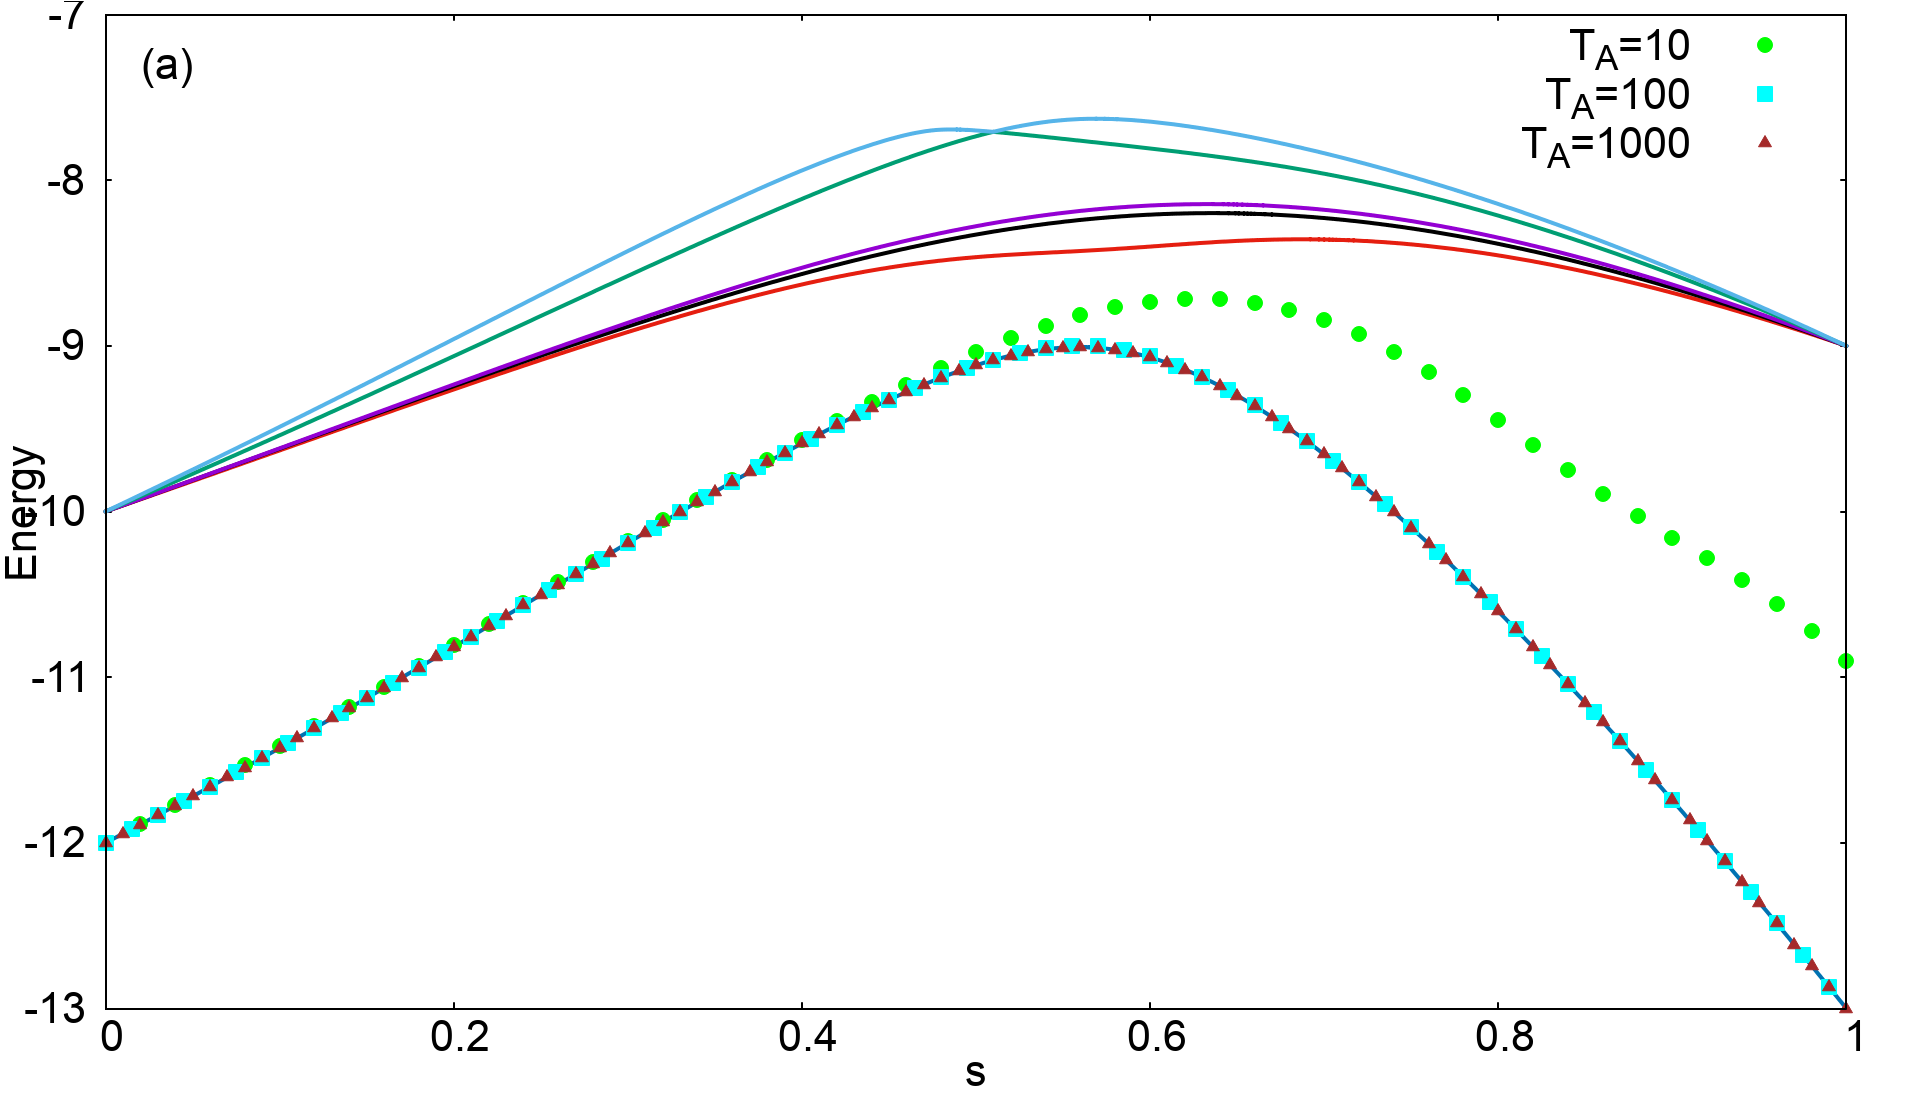
\includegraphics[scale=0.24]{733_s12_F_g0.png}
\caption{The energy spectrum and energy expectation values for the instantaneous state of problem 733, after adding the ferromagnetic trigger with g=0.5, for the three annealing times. $\Delta_{min}$ was found to be 0.5779, while $p$=0.9996 for $T_A$=100. }
\label{fig:f1}
\end{figure}
\begin{figure}[H]
\centering 
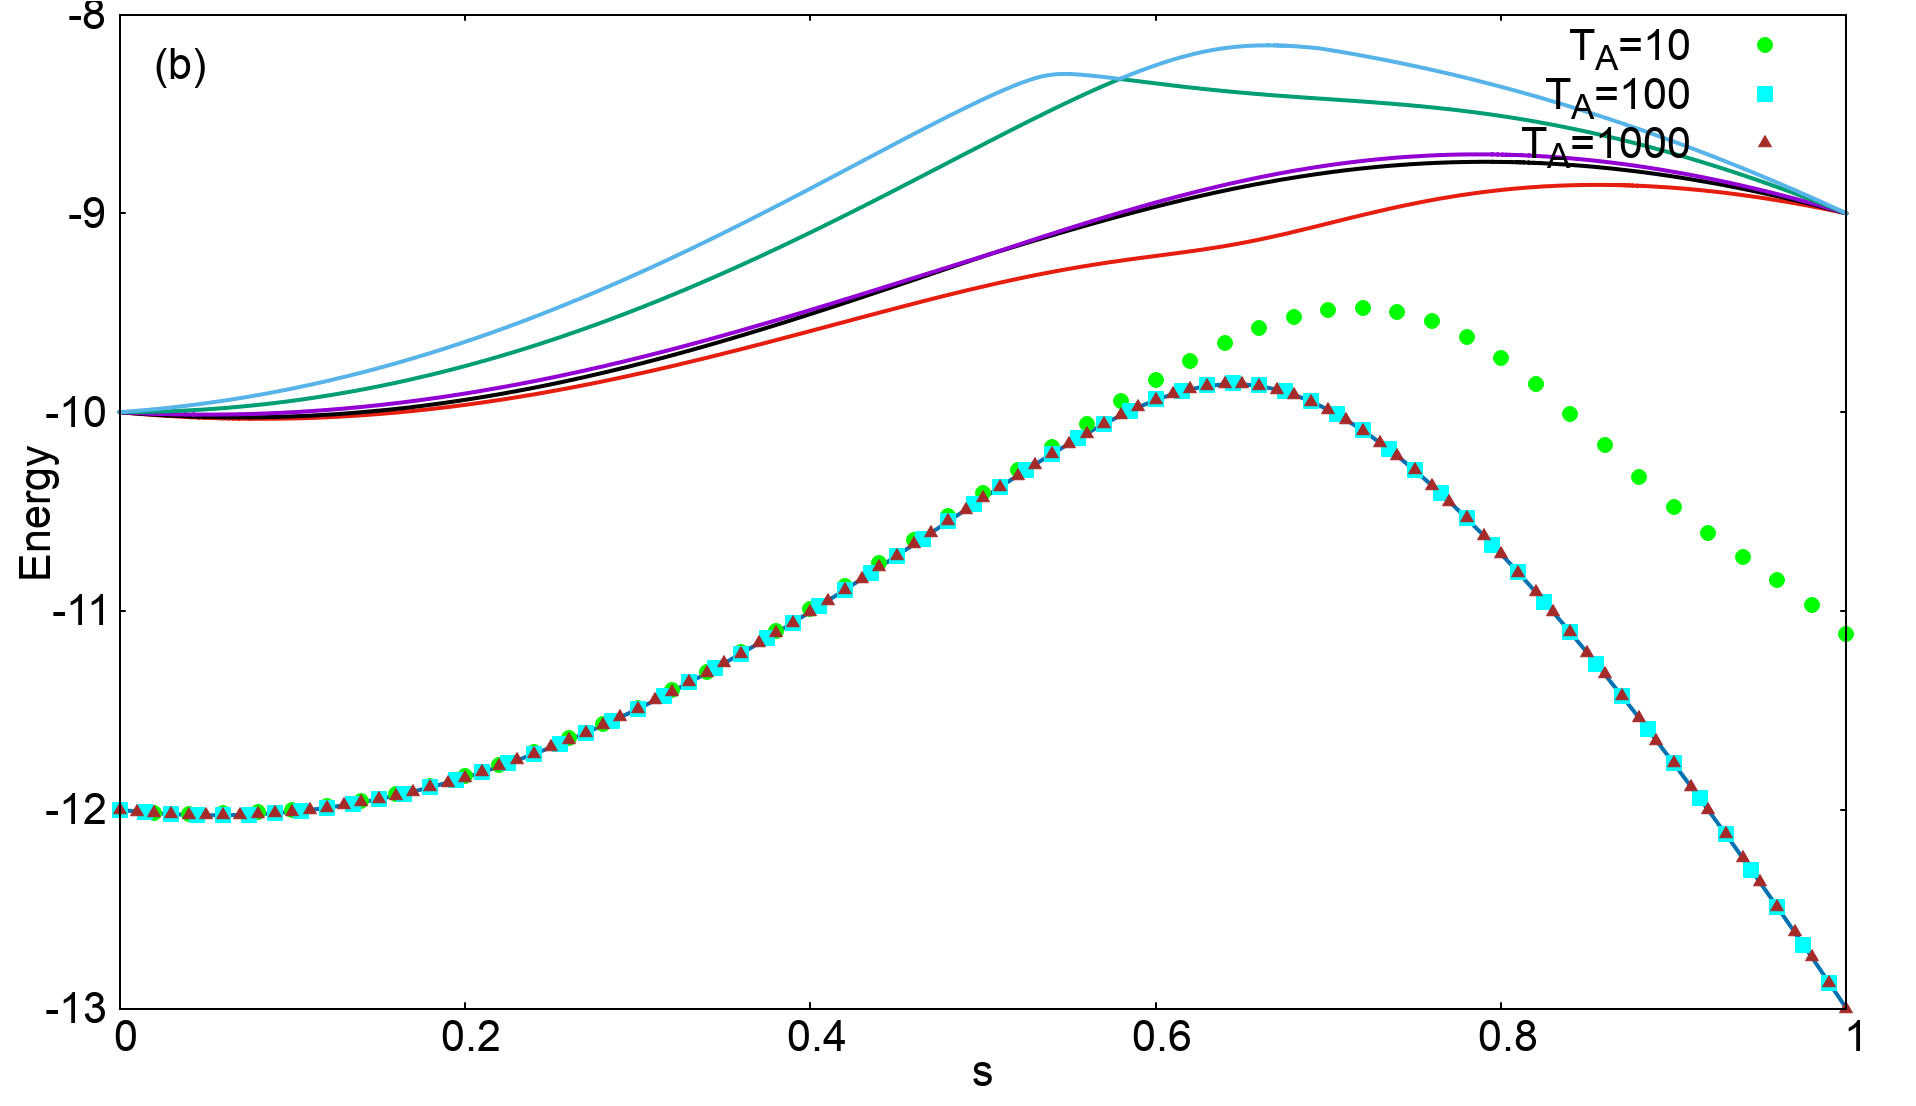
\includegraphics[scale=0.24]{733_s12_F_g1.png}
\caption{The energy spectrum and energy expectation values for the instantaneous state of problem 733, after adding the ferromagnetic trigger with g=1, for the three annealing times. $\Delta_{min}$ was found to be 0.6908, while $p$=0.9998 for $T_A$=100.}
\label{fig:f2}
\end{figure}
\begin{figure}[H]
\centering 
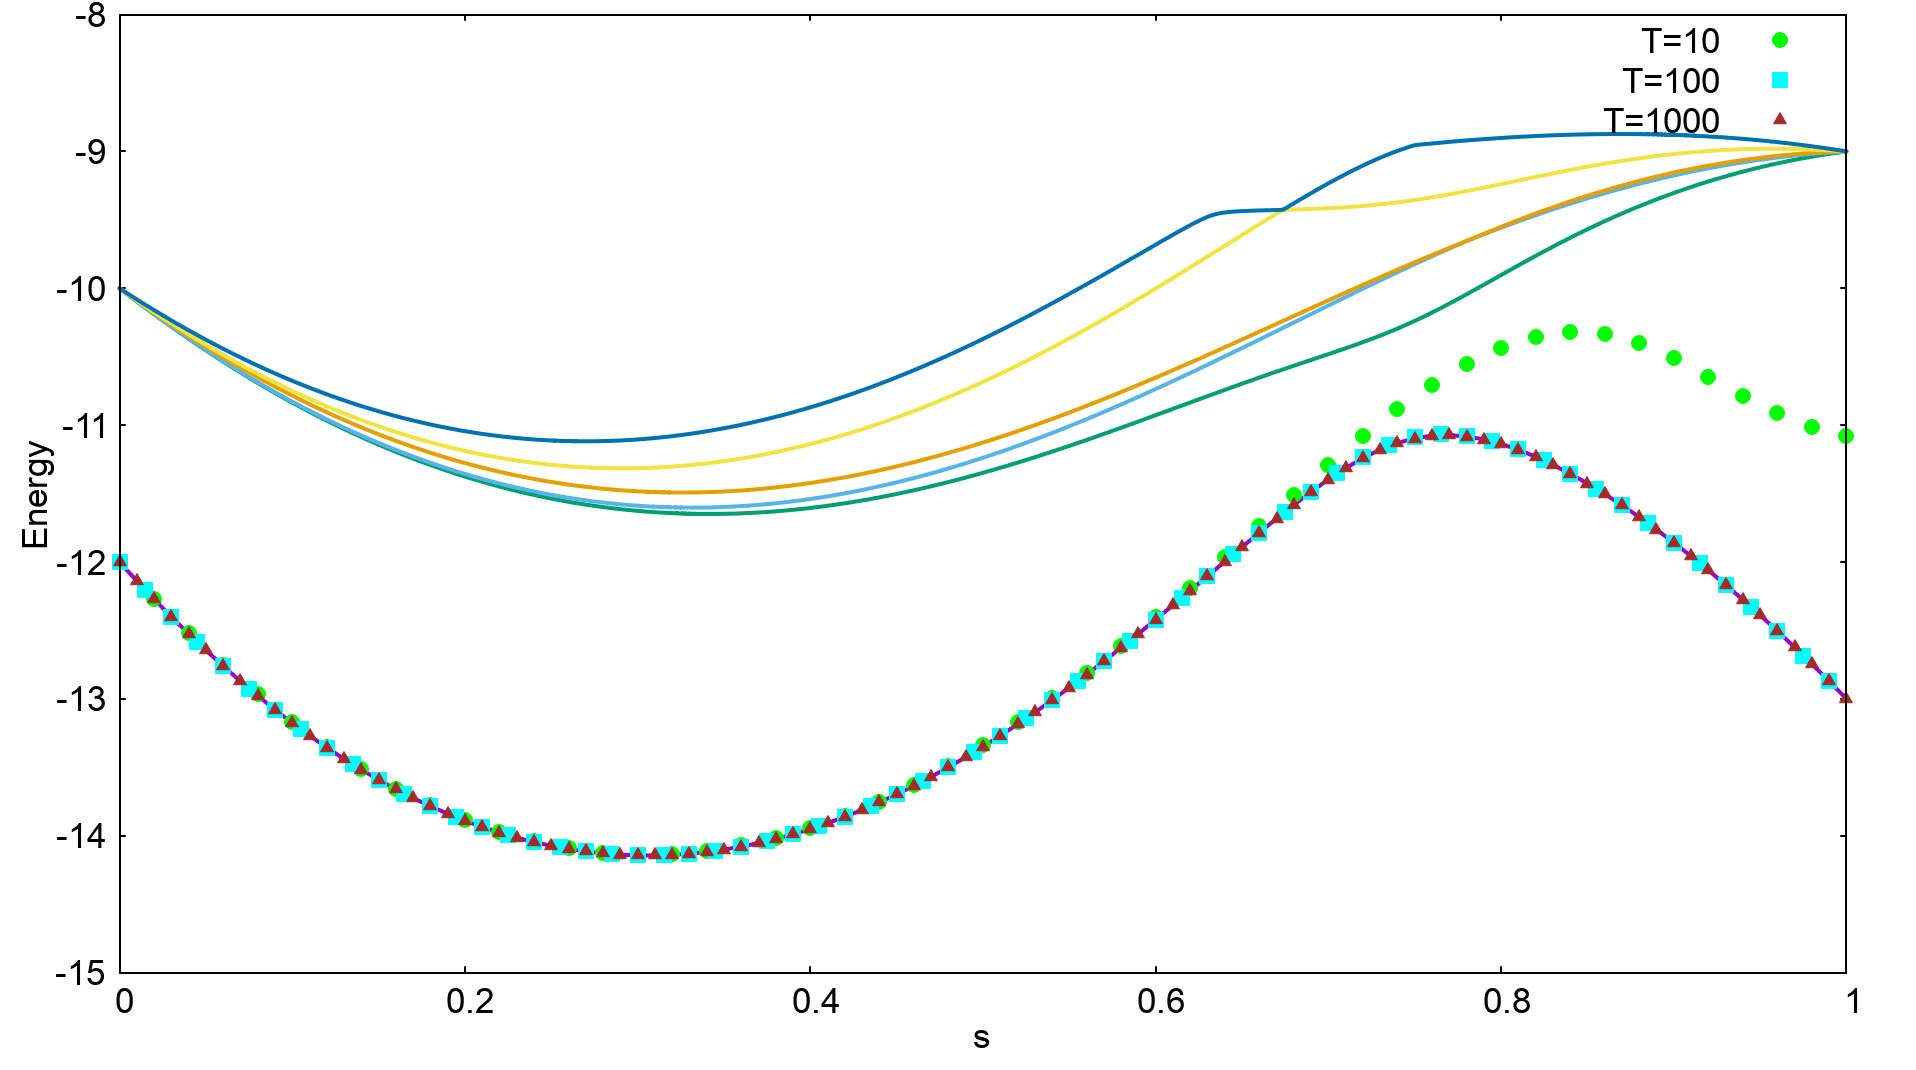
\includegraphics[scale=0.24]{733_s12_F_g2.png}
\caption{The energy spectrum and energy expectation values for the instantaneous state of problem 733, after adding the ferromagnetic trigger with g=2, for the three annealing times. $\Delta_{min}$ was found to be 0.8333, while $p$=0.9997 for $T_A$=100.}
\label{fig:f3}
\end{figure}
From these figures, it can be noted that compared to the original Hamiltonian, the minimum gap, $\Delta_{min}$ has increased for all the three case. Furthermore, the $\Delta_{min}$ becomes larger as the strength of the trigger Hamiltonian is increased from 0.5 to 2. \\
Secondly, the position of $\Delta_{min}$ is shifted more towards the right upon increasing the strength. Additionally, the concavity of the energy levels of the spectrum also increases with it. 
Finally, all the success probabilities upon adding the trigger are larger than the success probability of the original case, owing to the increase in the the minimum gaps. In general, the success probability also increases with increasing the strength of the trigger, though the final overlap also depends on the the exact energy spectrum. \\
Tab. (\ref{tab:f1}) shows a comparison of the minimum energy gaps and success probabilities for problem 733, before and after adding the trigger. 
\begin{table}[H]
\centering
\renewcommand{\arraystretch}{1.3}
\begin{tabular}{|c|c|c|c|c|}
\hline 
Problem 733 & Original Hamiltonian & Trigger=F, g=0.5 & Trigger=F, g=1 & Trigger=F, g=2 \\ 
\hline 
$\Delta_{min}$ & 0.4407 & 0.5779 & 0.6908 & 0.8333 \\ 
\hline 
p & 0.9944 & 0.9996 & 0.9998 & 0.9997 \\ 
\hline 
s value at $\Delta_{min}$ & 0.459 & 0.552 & 0.629 & 0.733 \\
\hline

\end{tabular} 
\caption{A comparison of the minimum energy gaps and the success probabilities for $T_A$=100, between the original Hamiltonian for problem 733 and that after adding the ferromagnetic trigger (F) with different strengths. The minimum gaps become larger as the strength of the ferromagnetic trigger is increased. The success probabilities are increased as a result. The value of s corresponding to the position of the minimum gap also becomes larger.}
\label{tab:f1}
\end{table}

Next, we focus on problem 950, which had a small success probability for the original Hamiltonian. Figs. (\ref{fig:f4}), (\ref{fig:f5}), (\ref{fig:f6}) show the energy spectra and the energy expectation values for the instantaneous state, upon adding the ferromagnetic trigger with g= 0.5, 1 and 2 respectively. 
\begin{figure}[H]
\centering 
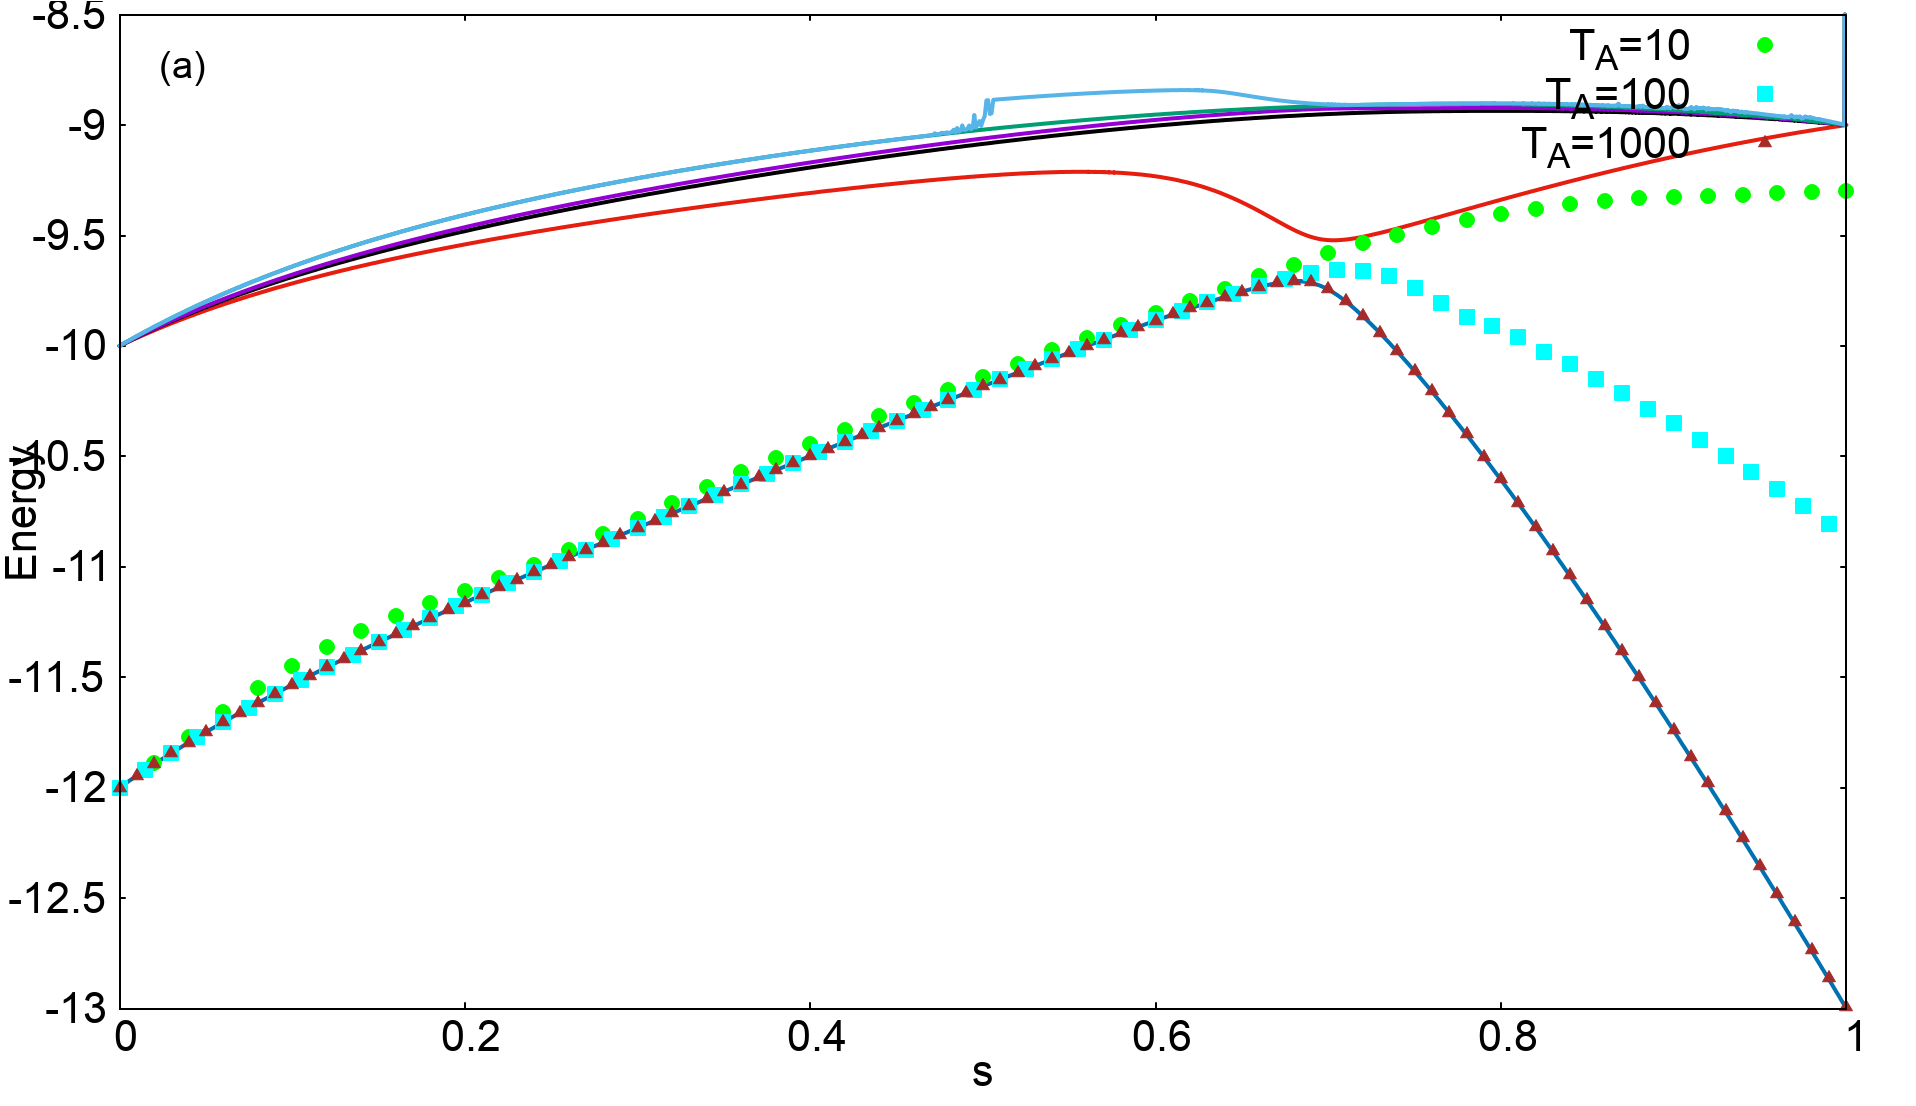
\includegraphics[scale=0.24]{950_s12_F_g0.png}
\caption{The energy spectrum and energy expectation values for the instantaneous state of problem 950, after adding the ferromagnetic trigger with g=0.5, for the three annealing times. $\Delta_{min}$ was found to be 0.2074, while $p$=0.4650 for $T_A$=100.}
\label{fig:f4}
\end{figure}

\begin{figure}[H]
\centering 
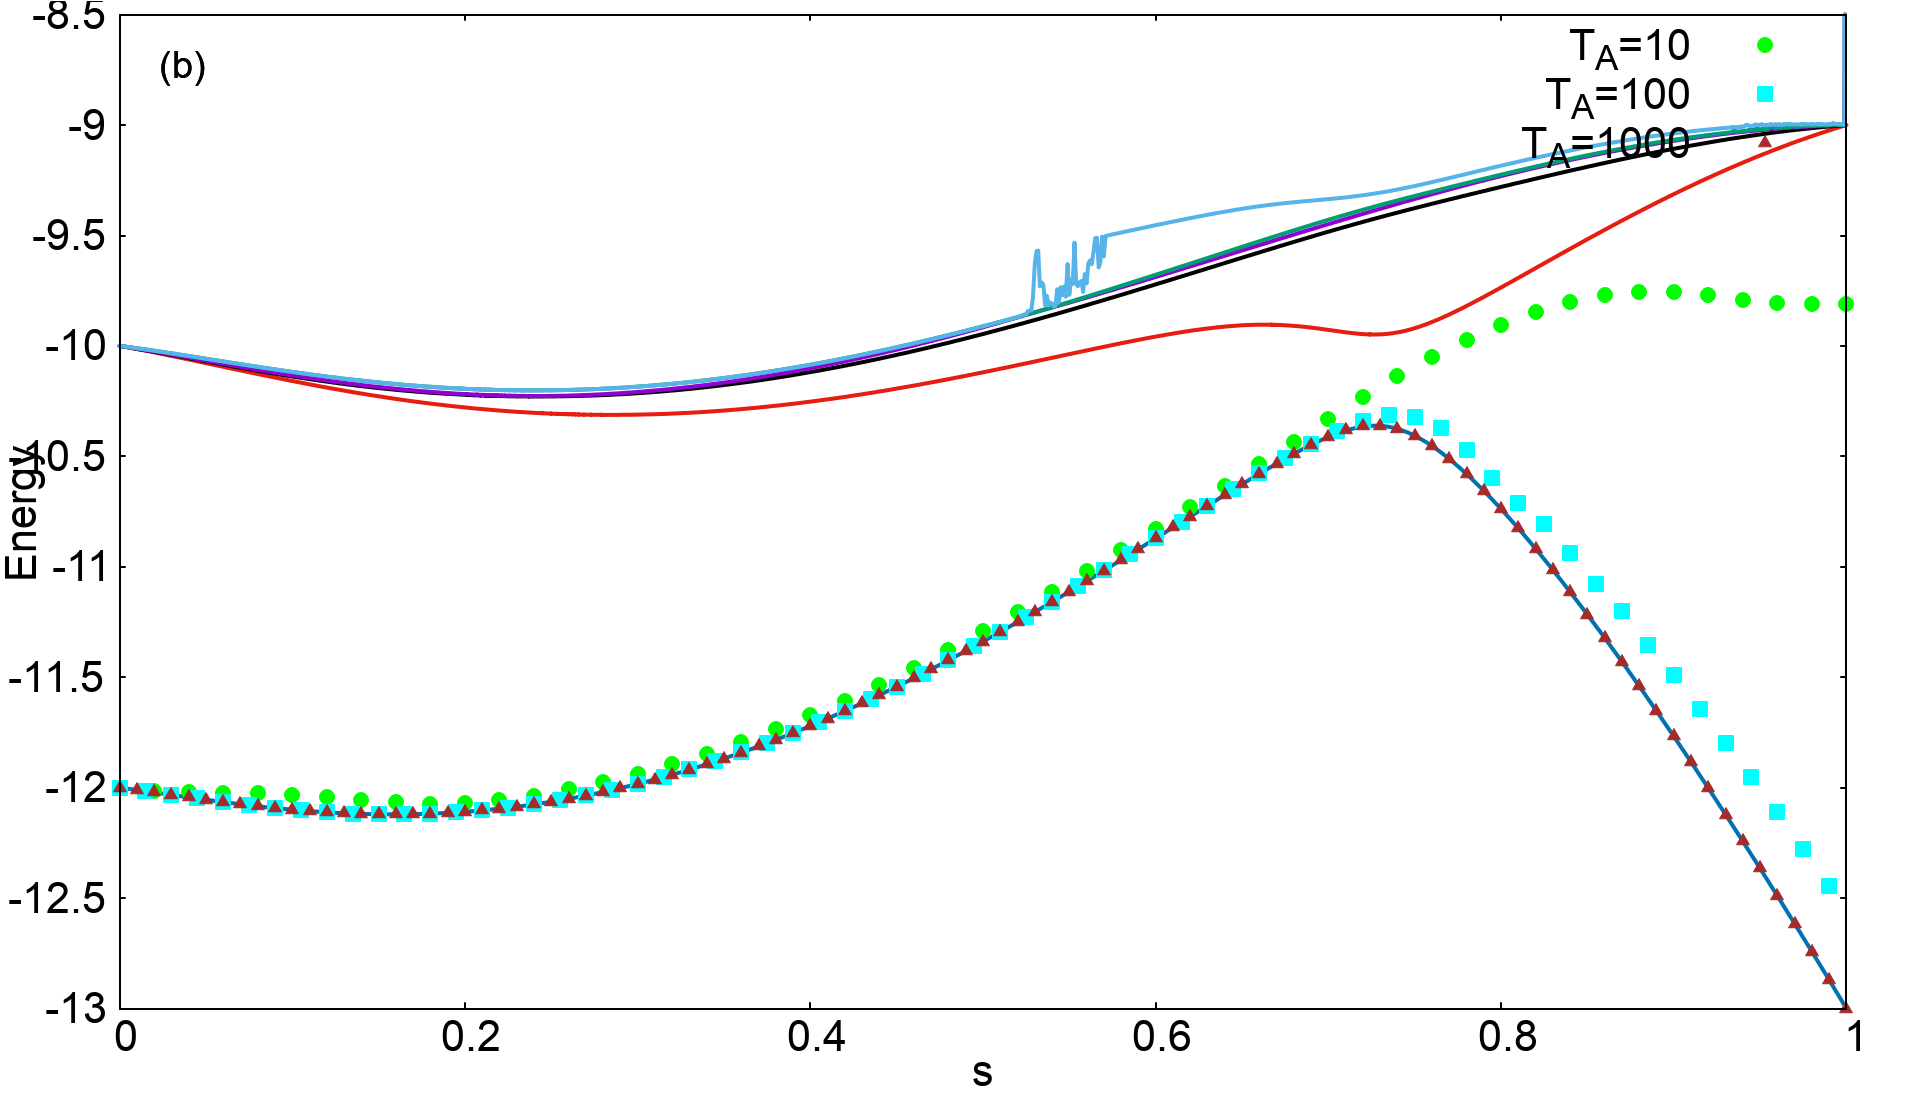
\includegraphics[scale=0.24]{950_s12_F_g1.png}
\caption{The energy spectrum and energy expectation values for the instantaneous state of problem 950, after adding the ferromagnetic trigger with g=1, for the three annealing times. $\Delta_{min}$ was found to be 0.4129, while $p$=0.8889 for $T_A$=100.}
\label{fig:f5}
\end{figure}
For this case too, the minimum energy gaps were found to have increased, leading to an improvement in the success probabilities. The improvements can be seen to become larger with increasing strengths of the trigger. The position of the minimum gap was again found to shift more rightwards in terms of the annealing parameter s upon increasing the strength, while the concavity of the energy levels increased. \\
\begin{figure}[H]
\centering 
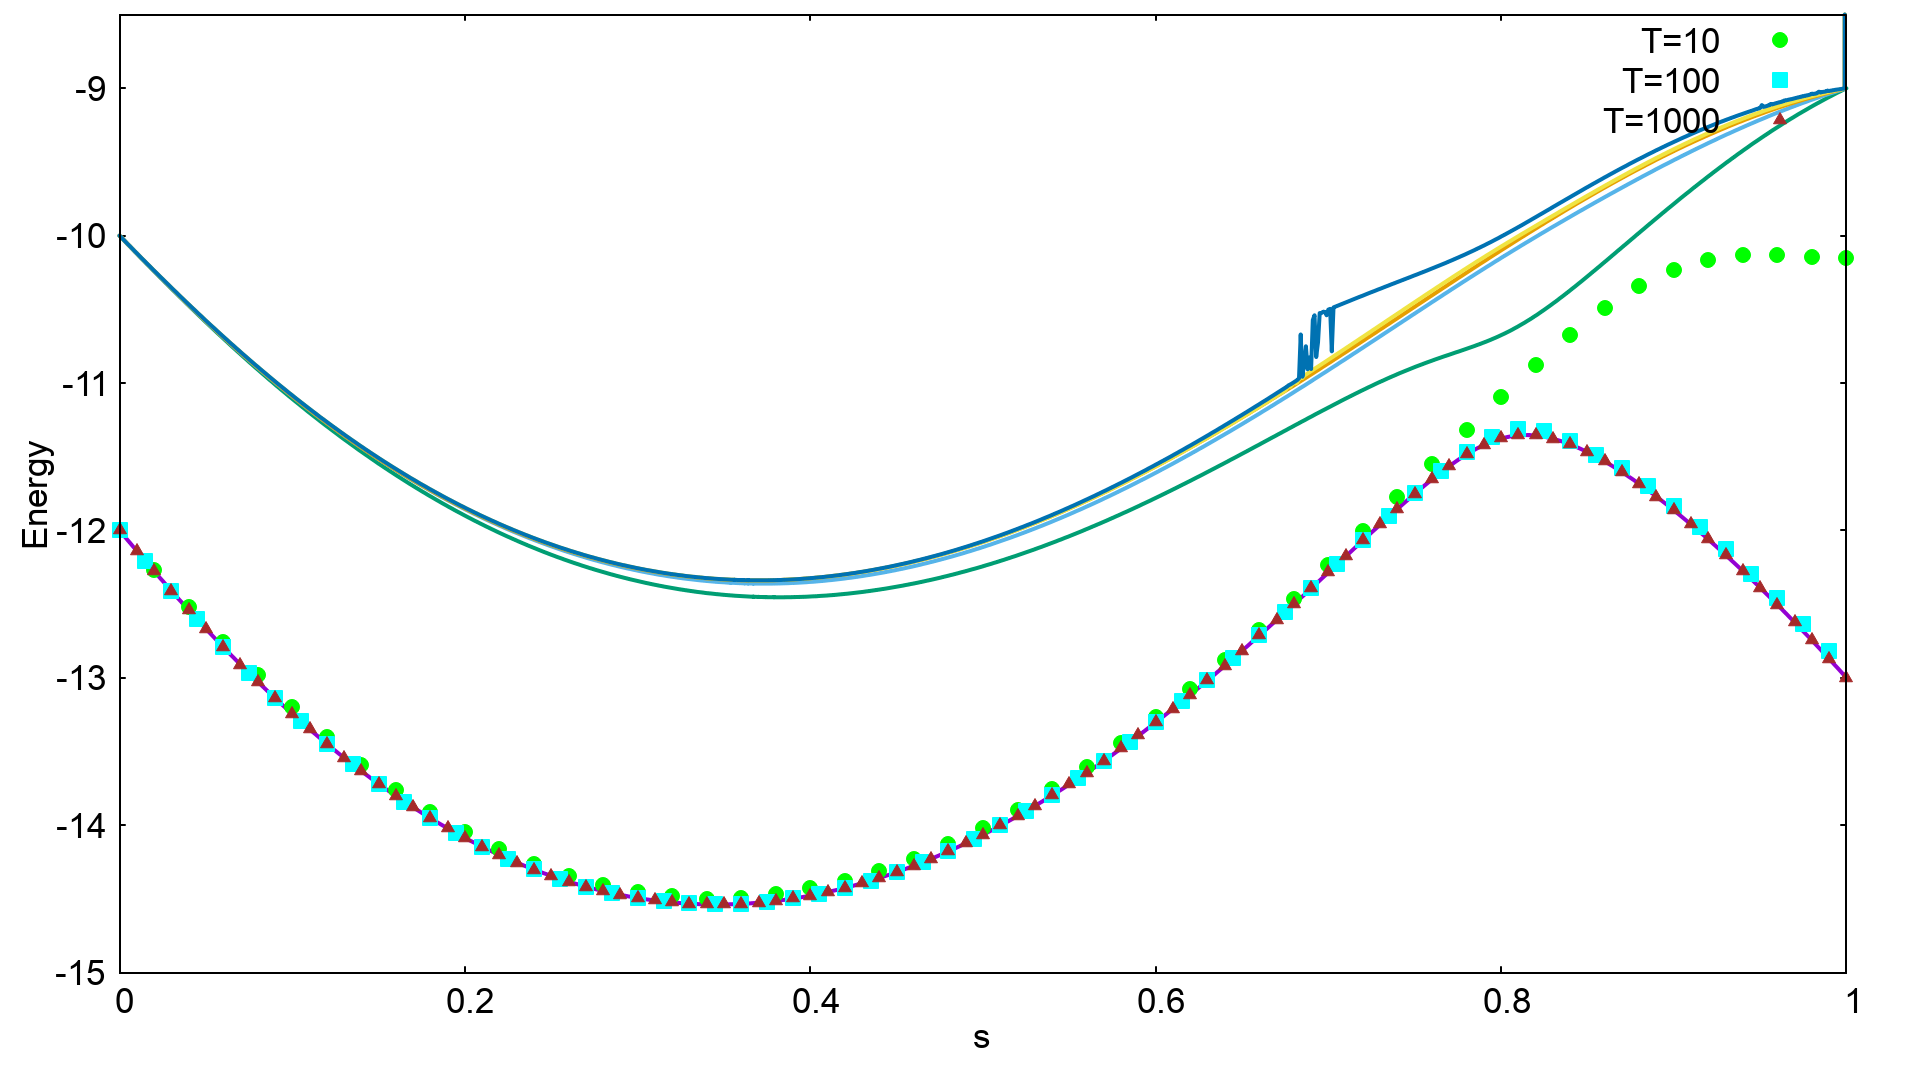
\includegraphics[scale=0.24]{950_s12_F_g2.png}
\caption{The energy spectrum and energy expectation values for the instantaneous state of problem 950, after adding the ferromagnetic trigger with g=2, for the three annealing times. $\Delta_{min}$ was found to be 0.6943, while $p$=0.9870 for $T_A$=100.}
\label{fig:f6}
\end{figure}
However, compared to the improvement in the success probability after adding the ferromagnetic trigger to problem 733, the improvement in problem 950 is significantly larger. Defining the relative success probability as the ratio of the success probability of a particular problem after adding the trigger ($p^F$) to the original success probability ($p^o$), for problem 733, the relative success probability at $T_A$=100 is 1.005 for g=2, while that for problem 950 is 67.6. In terms of the ratio of the minimum energy gaps, for problem 733, $\dfrac{\Delta_{min}^F}{\Delta_{min}^O}$=1.89, while for problem 950, it was found to be $\dfrac{\Delta_{min}^F}{\Delta_{min}^O}$=22.2. This can be understood as follows. For the original Hamiltonian for problem 733 and $T_A$=100, the system state always stays close to the ground state of the Hamiltonian (see Fig. \ref{fig:o2}), because of the large minimum energy gap. Therefore, even as adding the ferromagnetic trigger enlarges the minimum gap, there is not much scope of improvement for further increasing the overlap with the ground state. On the other hand, the original minimum energy gap in problem 950 is rather small. This causes the state of the system to shift most of its amplitude to the first excited state, thereby decreasing the overlap with ground state. Since the ferromagnetic trigger widens the minimum energy gap considerably in this case, the overlap with the ground state increases, resulting in a much larger relative success probability. 

Tab. (\ref{tab:f2}) gives a comparison of the minimum energy gaps and success probabilities for problem 950, before and after adding the trigger.
\begin{table}[H]
\centering
\renewcommand{\arraystretch}{1.3}
\begin{tabular}{|c|c|c|c|c|}
\hline 
Problem 950 & Original Hamiltonian & Trigger=F, g=0.5 & Trigger=F, g=1 & Trigger=F, g=2 \\ 
\hline 
$\Delta_{min}$ & 0.0312 & 0.2074 & 0.4129 & 0.6943 \\ 
\hline 
p & 0.0146 & 0.4650 & 0.8889 & 0.9870 \\ 
\hline 
s value at $\Delta_{min}$ & 0.665 & 0.691 & 0.727 & 0.793 \\
\hline

\end{tabular} 
\caption{A comparison of the minimum gaps and the success probabilities for $T_A$=100 between the original Hamiltonian for problem 950 and that after adding the  ferromagnetic trigger with different strengths. The minimum gaps become larger as the strength of the ferromagnetic trigger (F) is increased. The success probabilities are increased as a result. The value of s corresponding to the position of the minimum gap also becomes larger.}
\label{tab:f2}
\end{table}

Next, we consider problem 528 with intermediate success probability with original Hamiltonian. Figs. (\ref{fig:f7}), (\ref{fig:f8}) and (\ref{fig:f9}) show the energy spectra and the energy expectation values for the instantaneous state after adding the ferromagnetic trigger with strengths 0.5, 1 and 2 respectively.
\begin{figure}[H]
\centering 
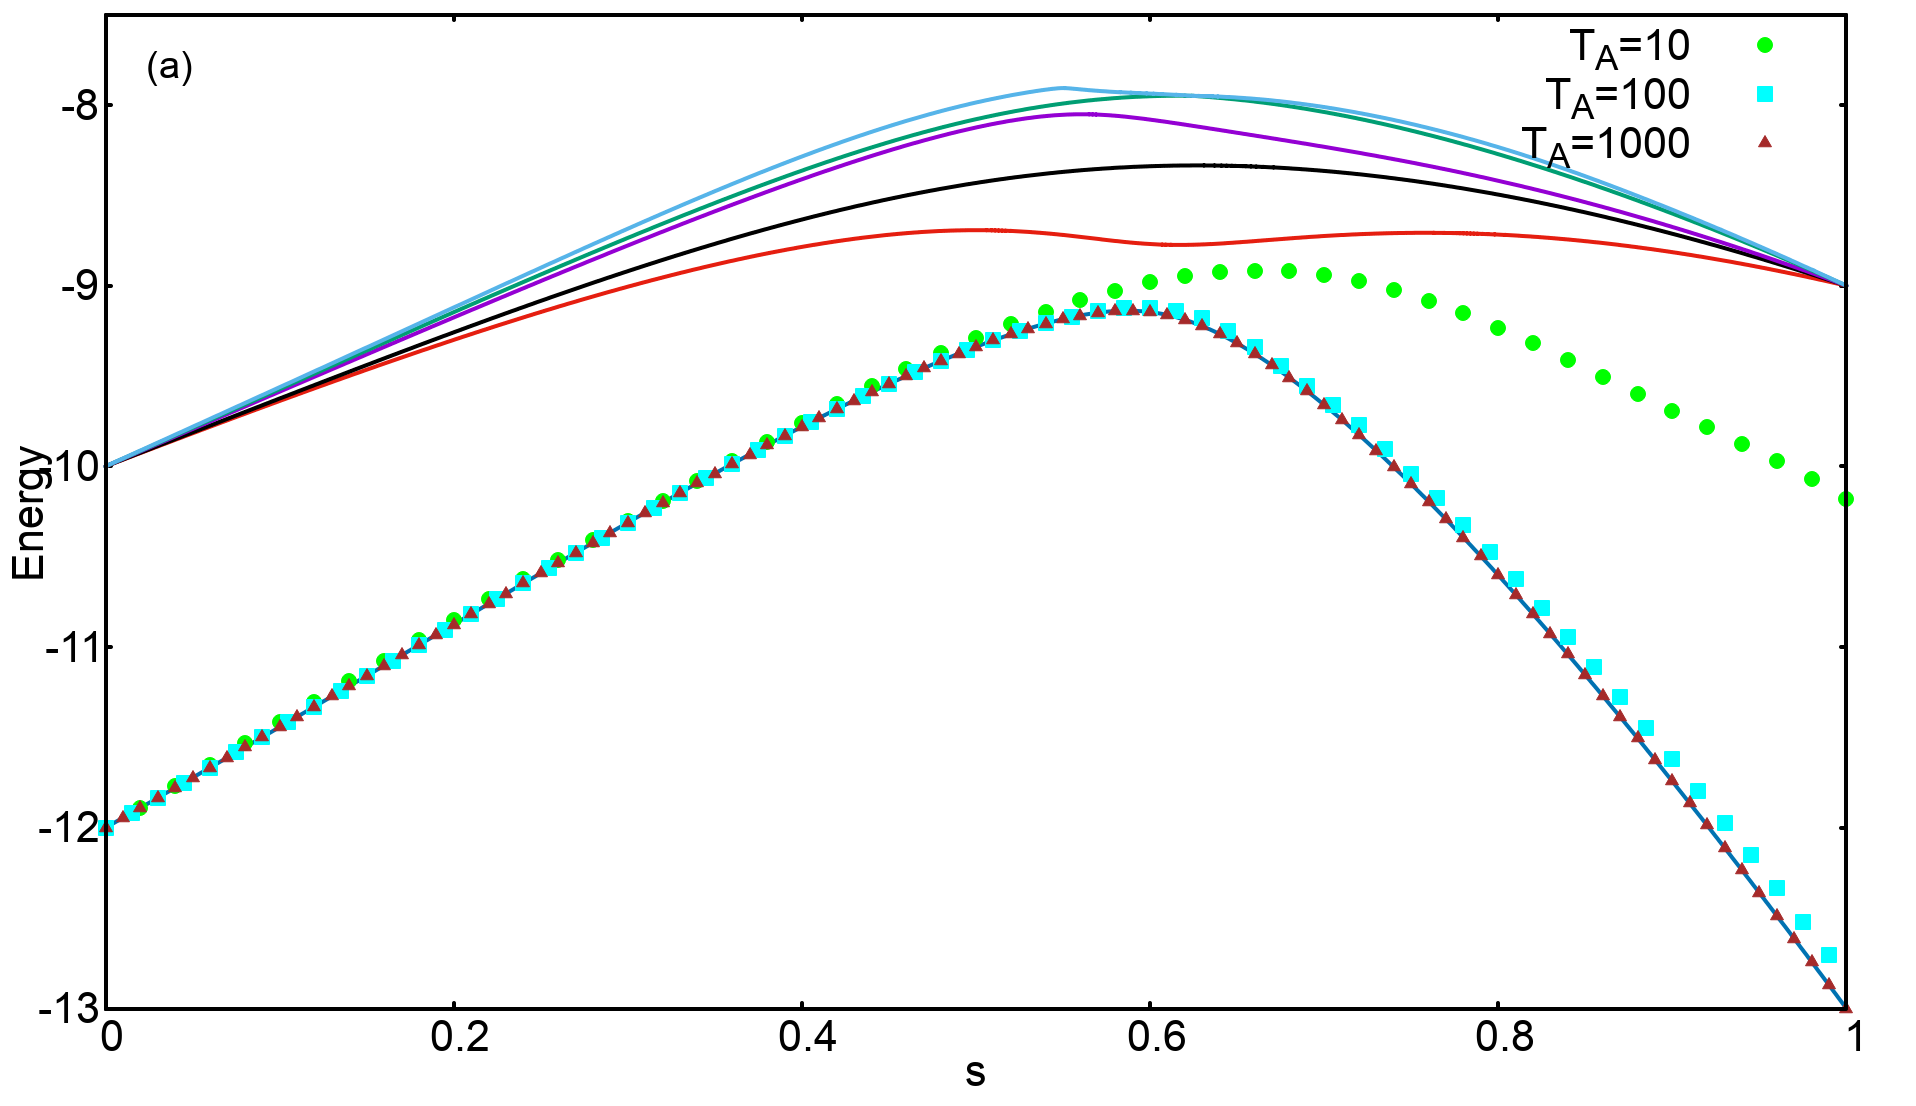
\includegraphics[scale=0.24]{528_s12_F_g0.png}
\caption{The energy spectrum and energy expectation values for the instantaneous state of problem 528, after adding the ferromagnetic trigger with g=0.5, for the three annealing times. $\Delta_{min}$ was found to be 0.3748, while $p$=0.9577 for $T_A$=100.}
\label{fig:f7}
\end{figure}
For this case too, the minimum energy gaps were found to have increased, leading to an improvement in the success probabilities. The improvements can be seen to become larger with increasing strengths of the trigger. The position of the minimum gap was again found to shift more rightwards in terms of the annealing parameter s upon increasing the strength, while the concavity of the energy levels of the spectrum increased. \\
\begin{figure}[H]
\centering 
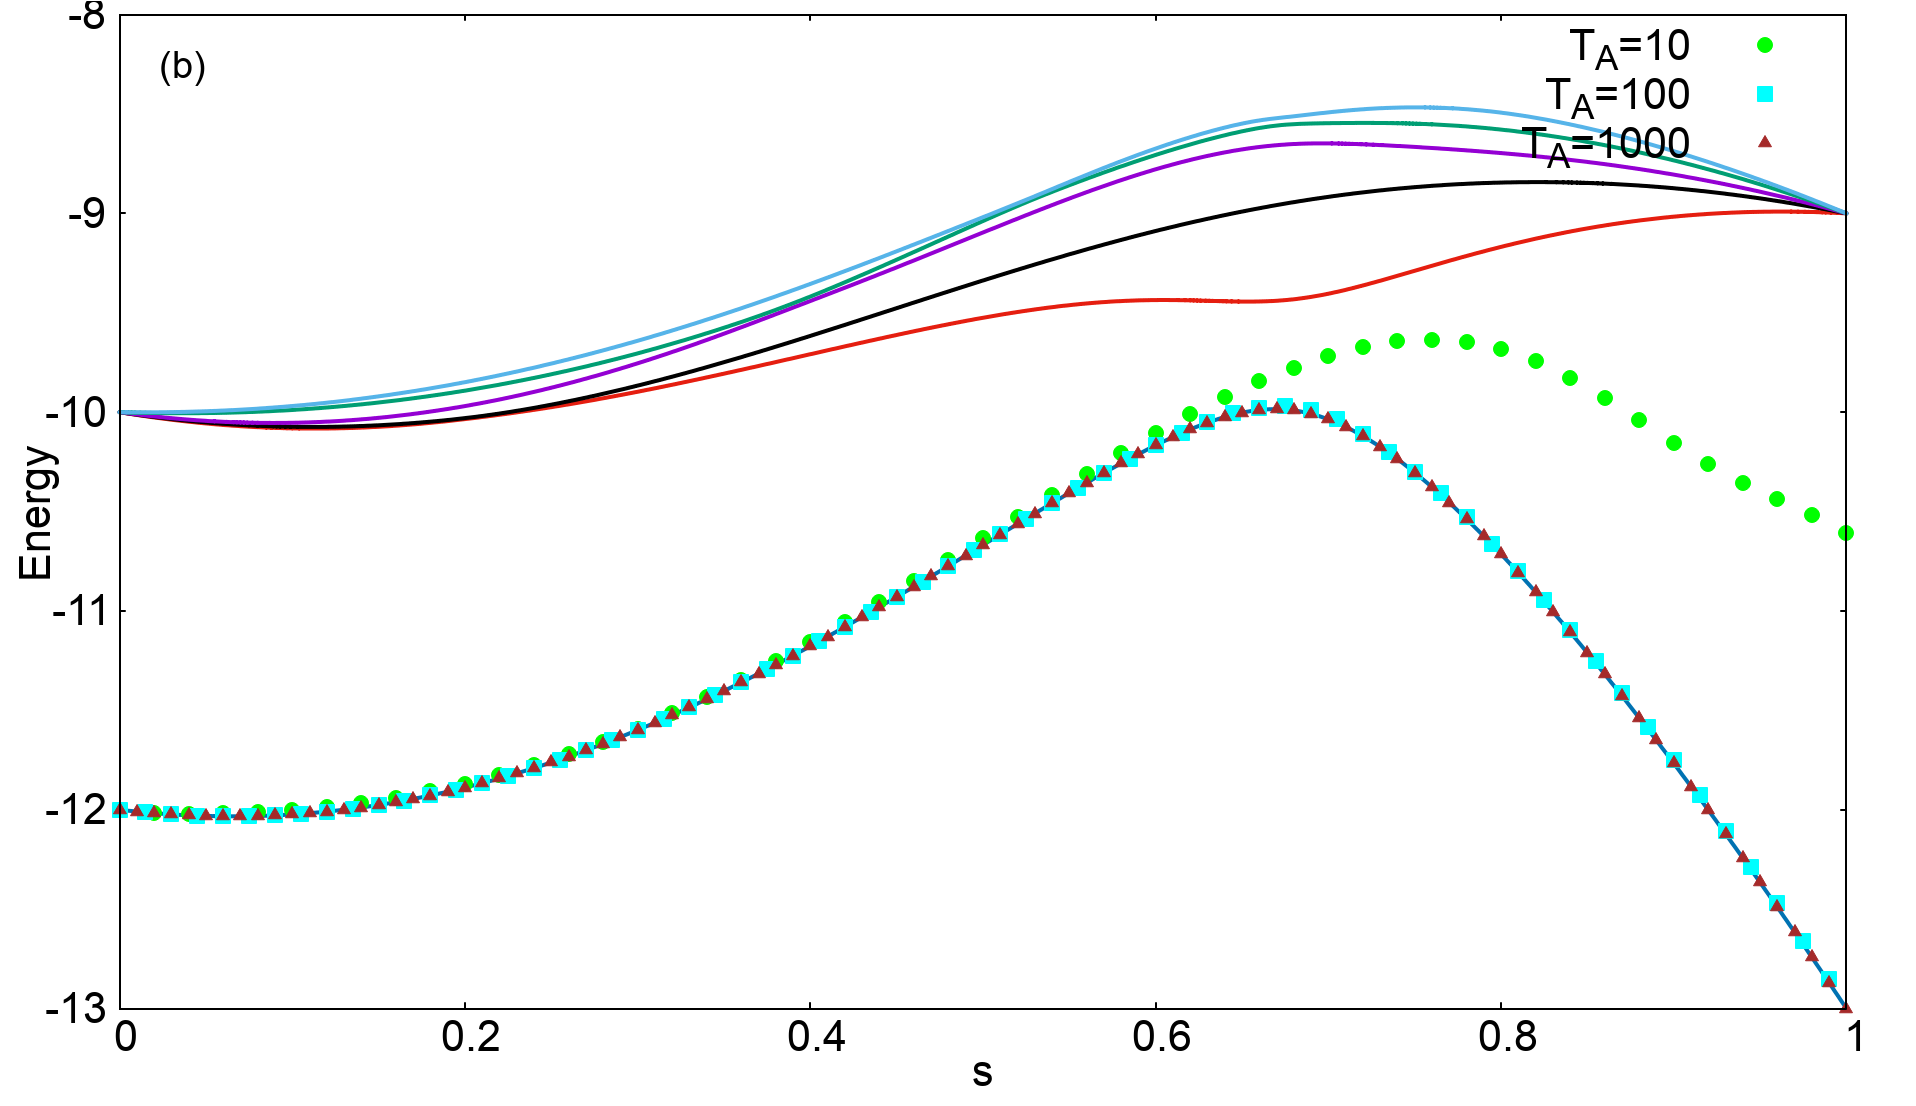
\includegraphics[scale=0.24]{528_s12_F_g1.png}
\caption{The energy spectrum and energy expectation values for the instantaneous state of problem 528, after adding the ferromagnetic trigger with g=1, for the three annealing times. $\Delta_{min}$ was found to be 0.5439, while $p$=0.9945 for $T_A$=100.}
\label{fig:f8}
\end{figure}
\begin{figure}[H]
\centering 
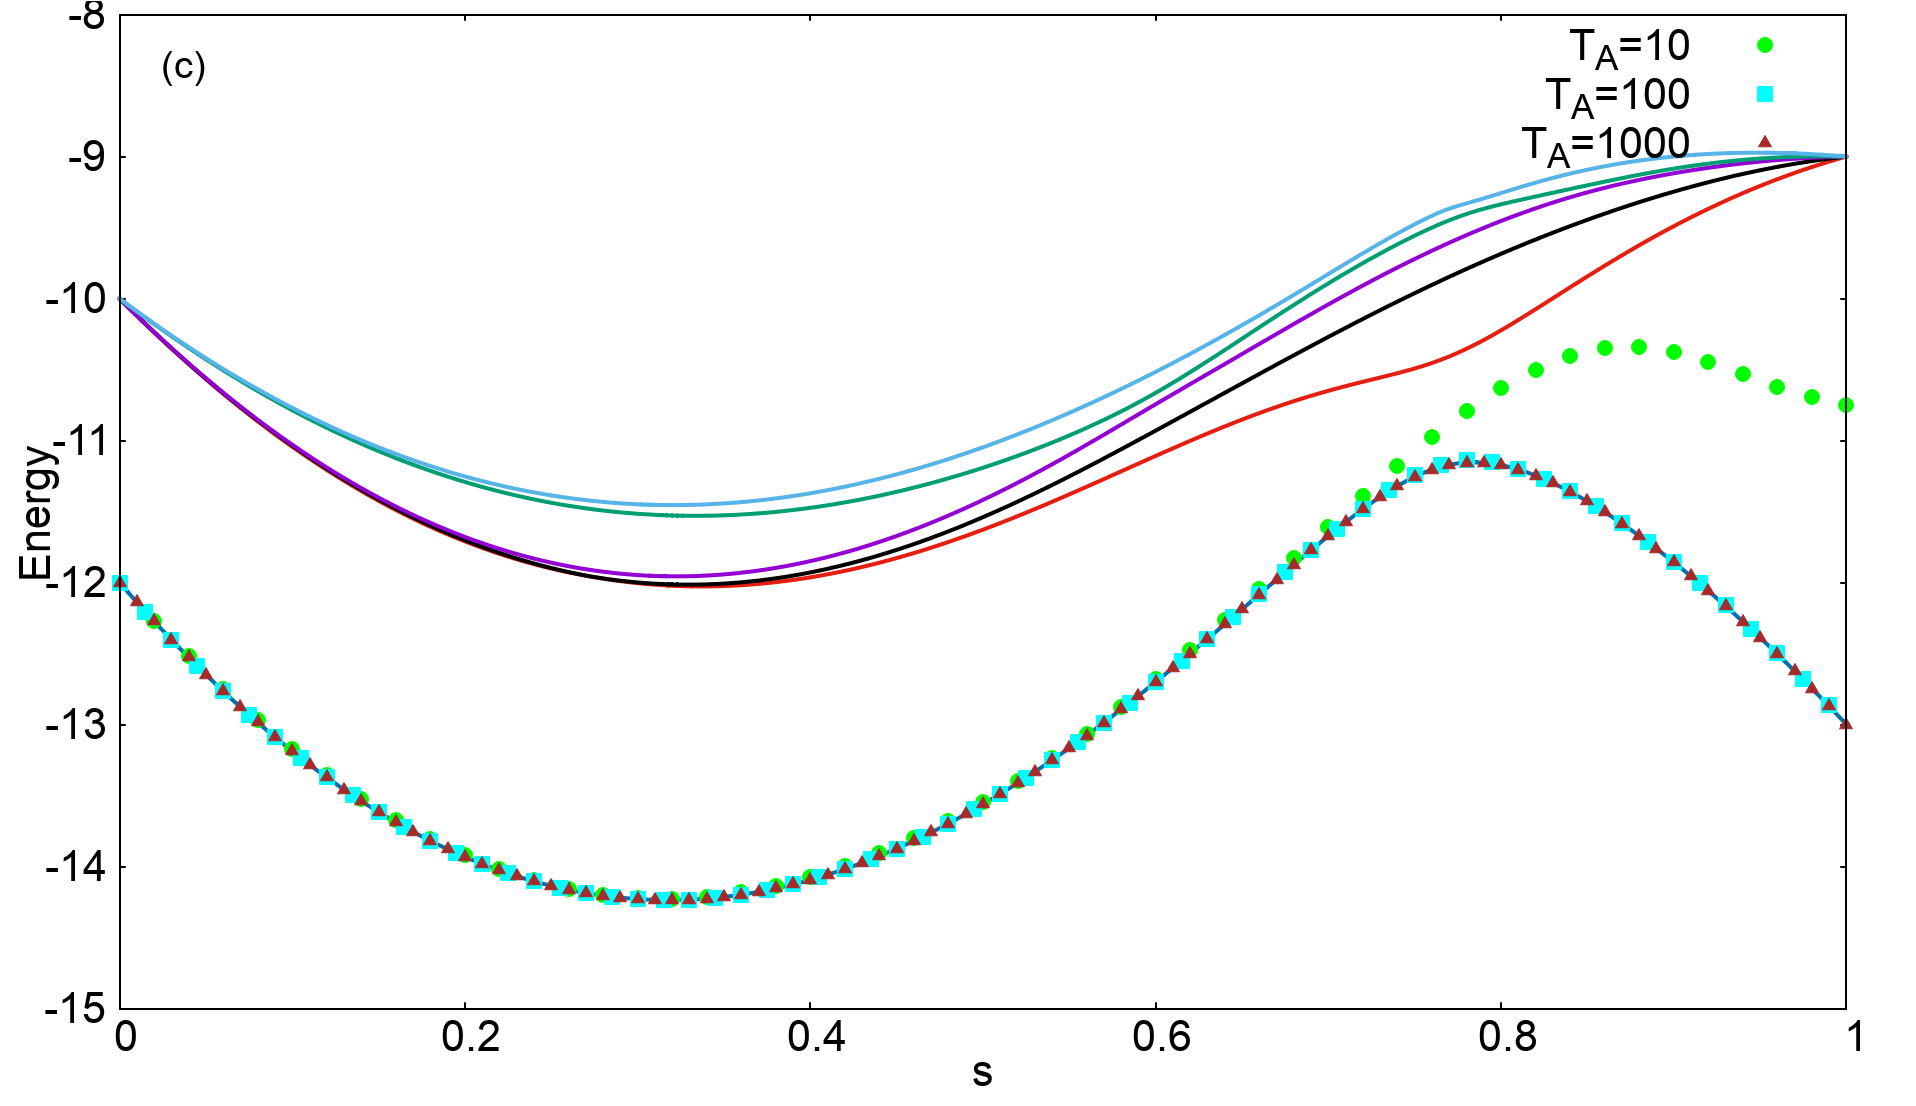
\includegraphics[scale=0.24]{528_s12_F_g2.png}
\caption{The energy spectrum and energy expectation values for the instantaneous state of problem 528, after adding the ferromagnetic trigger with g=2, for the three annealing times. $\Delta_{min}$ was found to be 0.7512, while $p$=0.9981 for $T_A$=100.}
\label{fig:f9}
\end{figure}
The relative success ratio for this case,=1.91 , while $\dfrac{\Delta_{min}^F}{\Delta_{min}^O}$=4.77 at g=2. These values are also intermediate to those for problems 733 and 950.  Tab. (\ref{tab:f3}) shows a comparison of the success probabilities and the minimum gaps, between the original Hamiltonian and the Hamiltonian after adding the ferromagnetic trigger with different strengths.
\begin{table}[H]
\centering
\renewcommand{\arraystretch}{1.3}
\begin{tabular}{|c|c|c|c|c|}
\hline 
Problem 528 & Original Hamiltonian & Trigger=F, g=0.5 & Trigger=F, g=1 & Trigger=F, g=2 \\ 
\hline 
$\Delta_{min}$ & 0.1573 & 0.3748 & 0.5439 & 0.7512 \\ 
\hline 
p & 0.5199 & 0.9577 & 0.9945 & 0.9981 \\ 
\hline 
s value at $\Delta_{min}$ & 0.514 & 0.595 & 0.665 & 0.760 \\
\hline

\end{tabular} 
\caption{A comparison of the minimum energy gaps and the success probabilities for $T_A$=100, between the original Hamiltonian for problem 528 and that after adding the ferromagnetic trigger (F) with different strengths. The minimum gaps become larger as the strength of the ferromagnetic trigger is increased. The success probabilities are increased as a result. The value of s corresponding to the position of the minimum gap also becomes larger.}
\label{tab:f3}
\end{table}
Next, the minimum energy gaps and the success probabilities were computed for all the 12-spin problems, before and after adding the ferromagnetic trigger, with g $\in$ \{0.5,1,2\}, for $T_A$ $\in$ \{10,100,1000\}. \\

Fig. (\ref{fig:f10}) shows the scatter plot of the minimum energy gaps after adding the ferromagnetic trigger with different strengths against the original minimum energy gaps, for all the problems of the set.

\begin{figure}[H]
\centering 
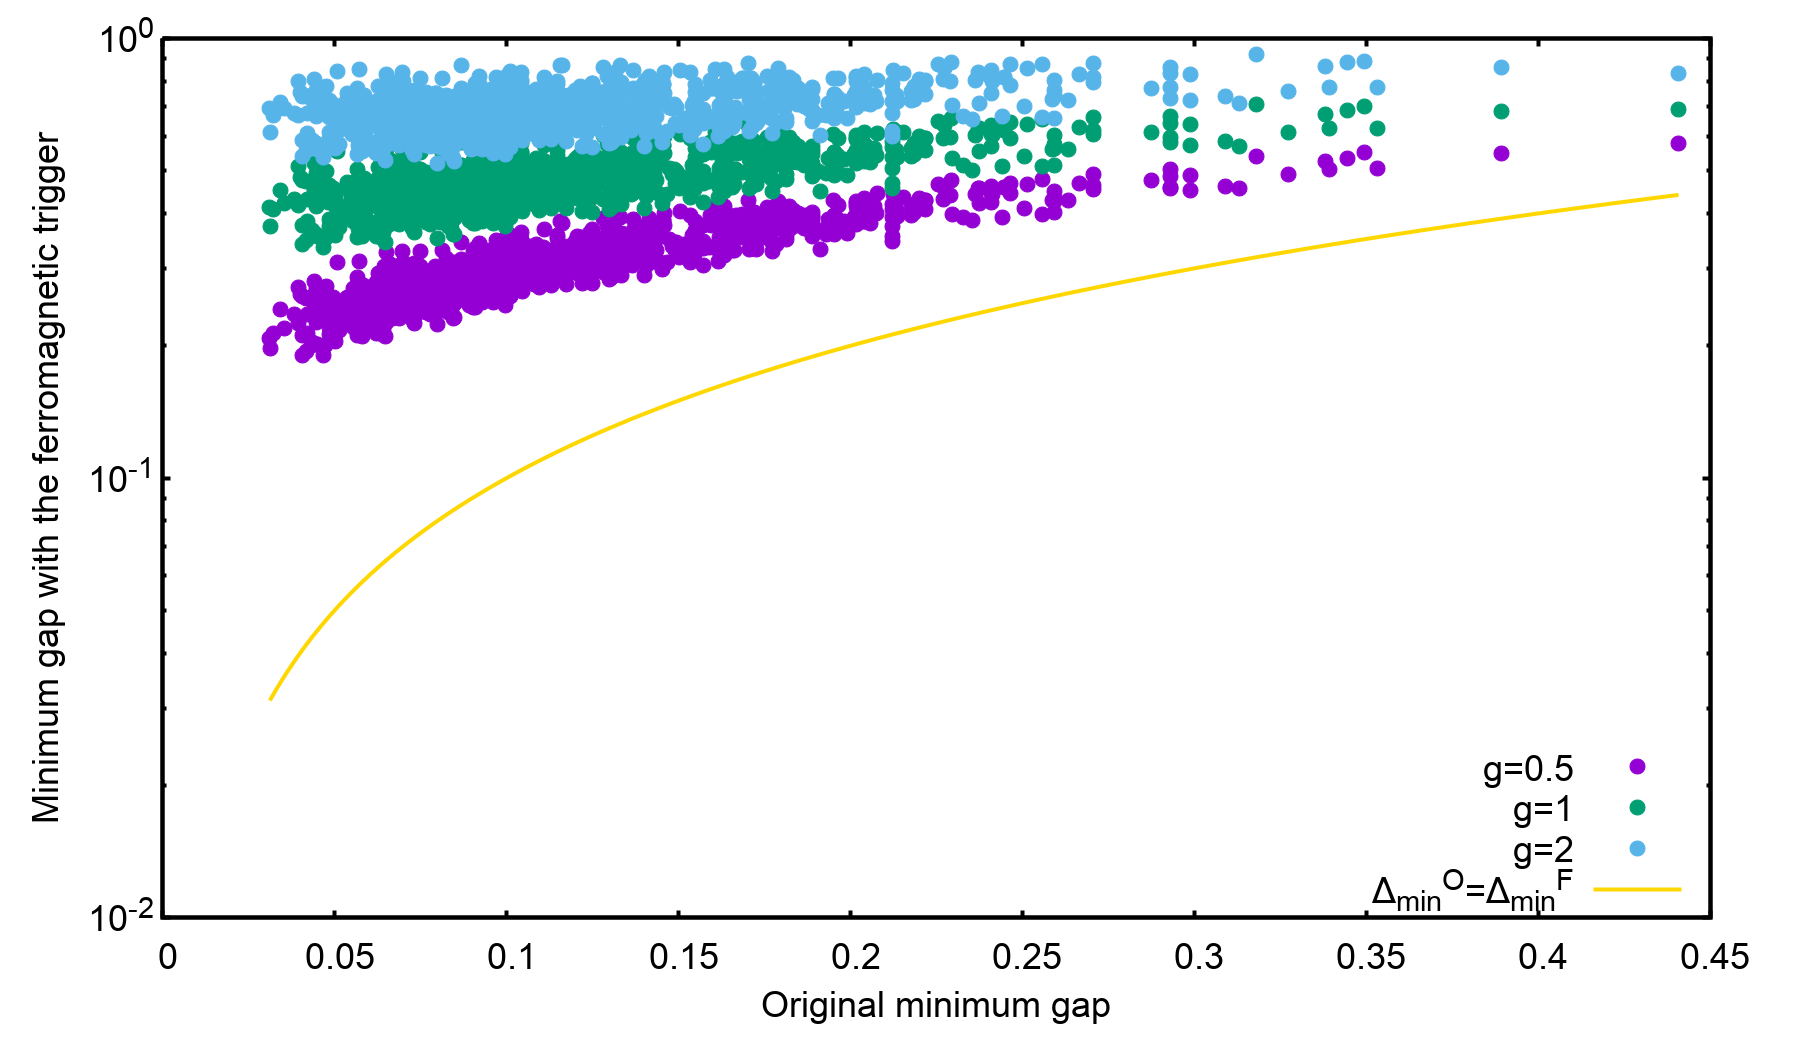
\includegraphics[scale=0.2]{Mingap_F_g0_1_2.png}
\caption{Scatter plot of the minimum gaps upon adding the ferromagnetic trigger with g $\in$ \{0.5,1,2\} against the original minimum energy gaps. The solid line represents the limit where the minimum gap remains unchanged.}
\label{fig:f10}
\end{figure}
With ferromagnetic trigger, all the minimum energy gaps were found to have increased, for  all the values of g. Furthermore, for all the problems, the gaps became even larger as the ferromagnetic trigger became stronger. It can also be noted that the enhancement in the minimum energy gaps is larger in cases with relatively small original minimum gaps, as was also seen by calculating $\dfrac{\Delta_{min}^F}{\Delta_{min}^O}$ for the three chosen problems (733, 950 and 528). 

For gauging the performance of the quantum annealing algorithm after adding the ferromagnetic trigger, scatter plots of the success probabilities after adding the ferromagnetic trigger against the original success probabilities have been shown in Figs. (\ref{fig:f11}), (\ref{fig:f12}) and (\ref{fig:f13}) corresponding to g= 0.5, 1 and 2 respectively.
\begin{figure}[H]
\centering 
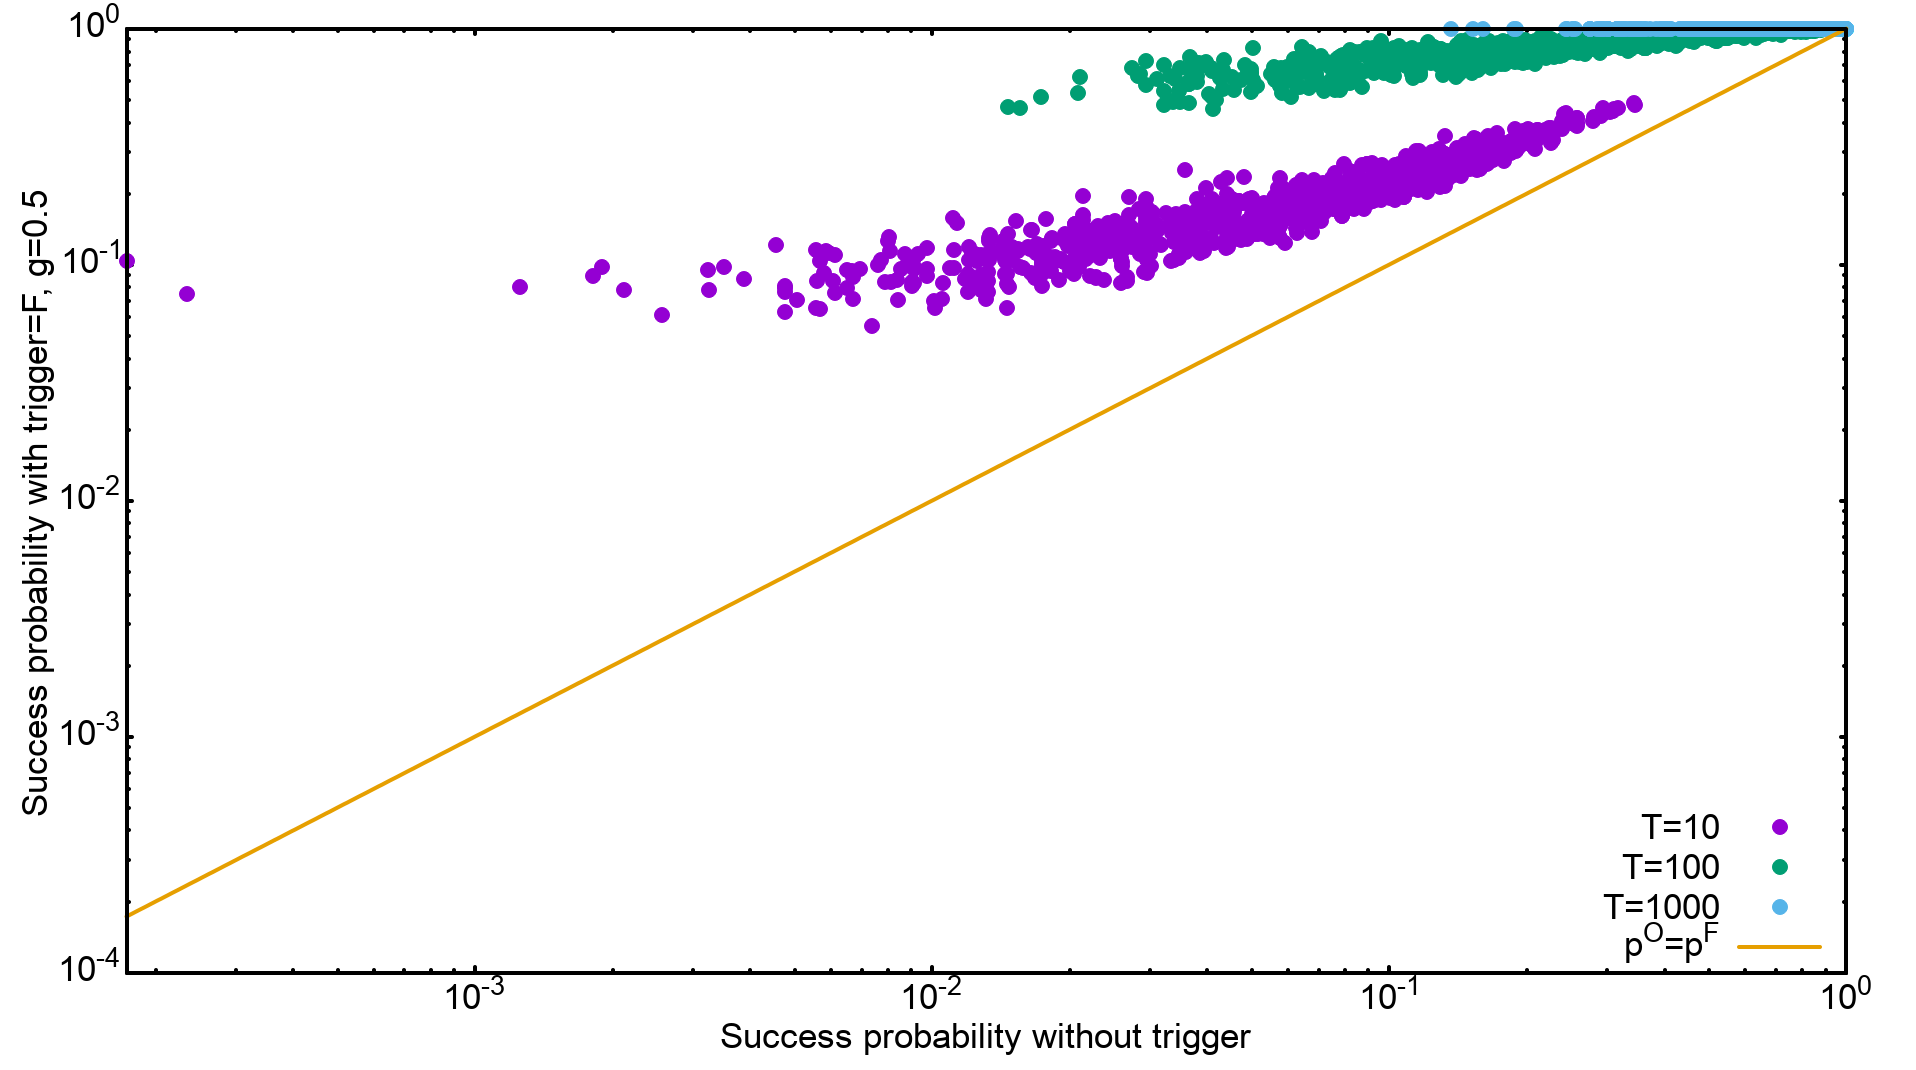
\includegraphics[scale=0.24]{Scatt_s12_F_g0.png}
\caption{Scatter plot for the success probability after adding ferromagnetic trigger with g=0.5 against the success probability of the original Hamiltonian, for annealing time $T_A \in \{10,100,1000\}$. The solid line represents the limit where the success probability remains unchanged.}
\label{fig:f11}
\end{figure}
\begin{figure}[H]
\centering
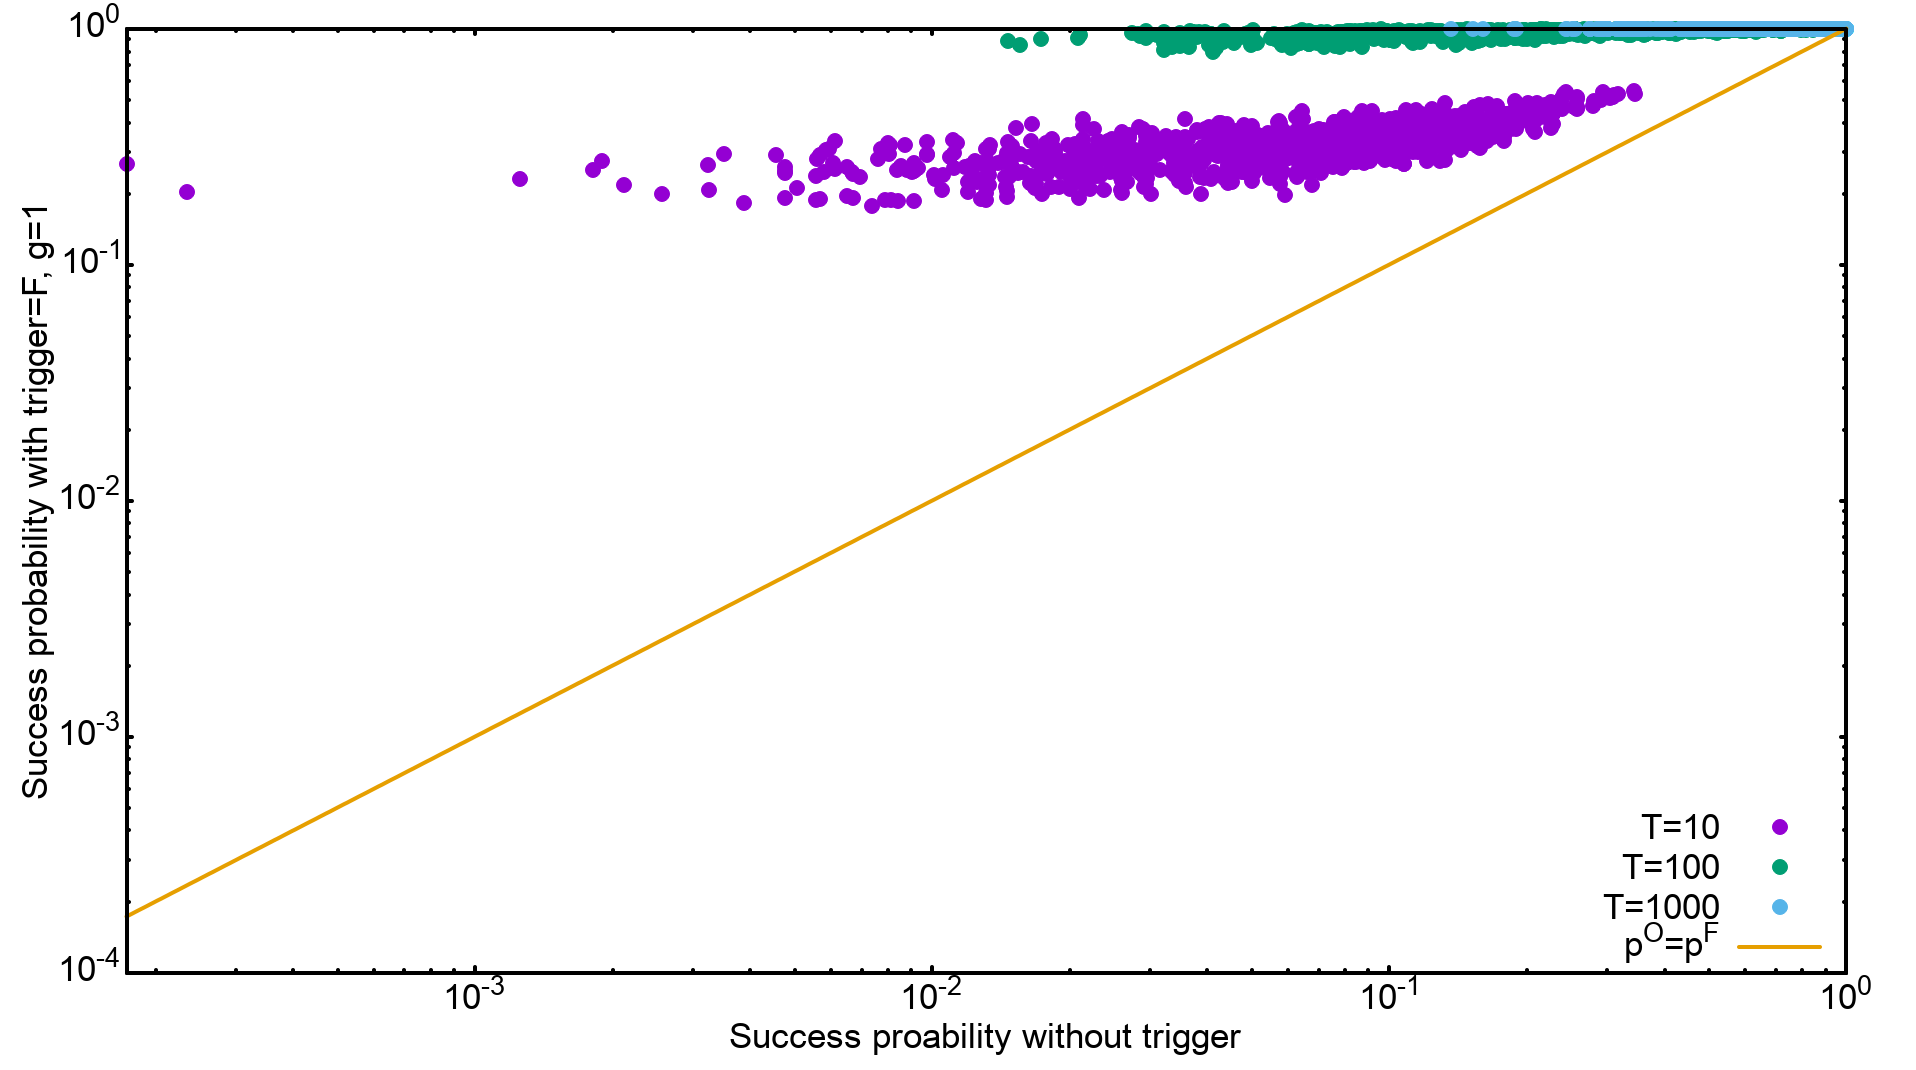
\includegraphics[scale=0.24]{Scatt_s12_F_g1.png}
\caption{Scatter plot for the success probability after adding ferromagnetic trigger with g=1 against the success probability of the original Hamiltonian, for annealing time $T_A \in \{10,100,1000\}$. The solid line represents the limit where the success probability remains unchanged.}
\label{fig:f12}
\end{figure}
\begin{figure}[H]
\centering
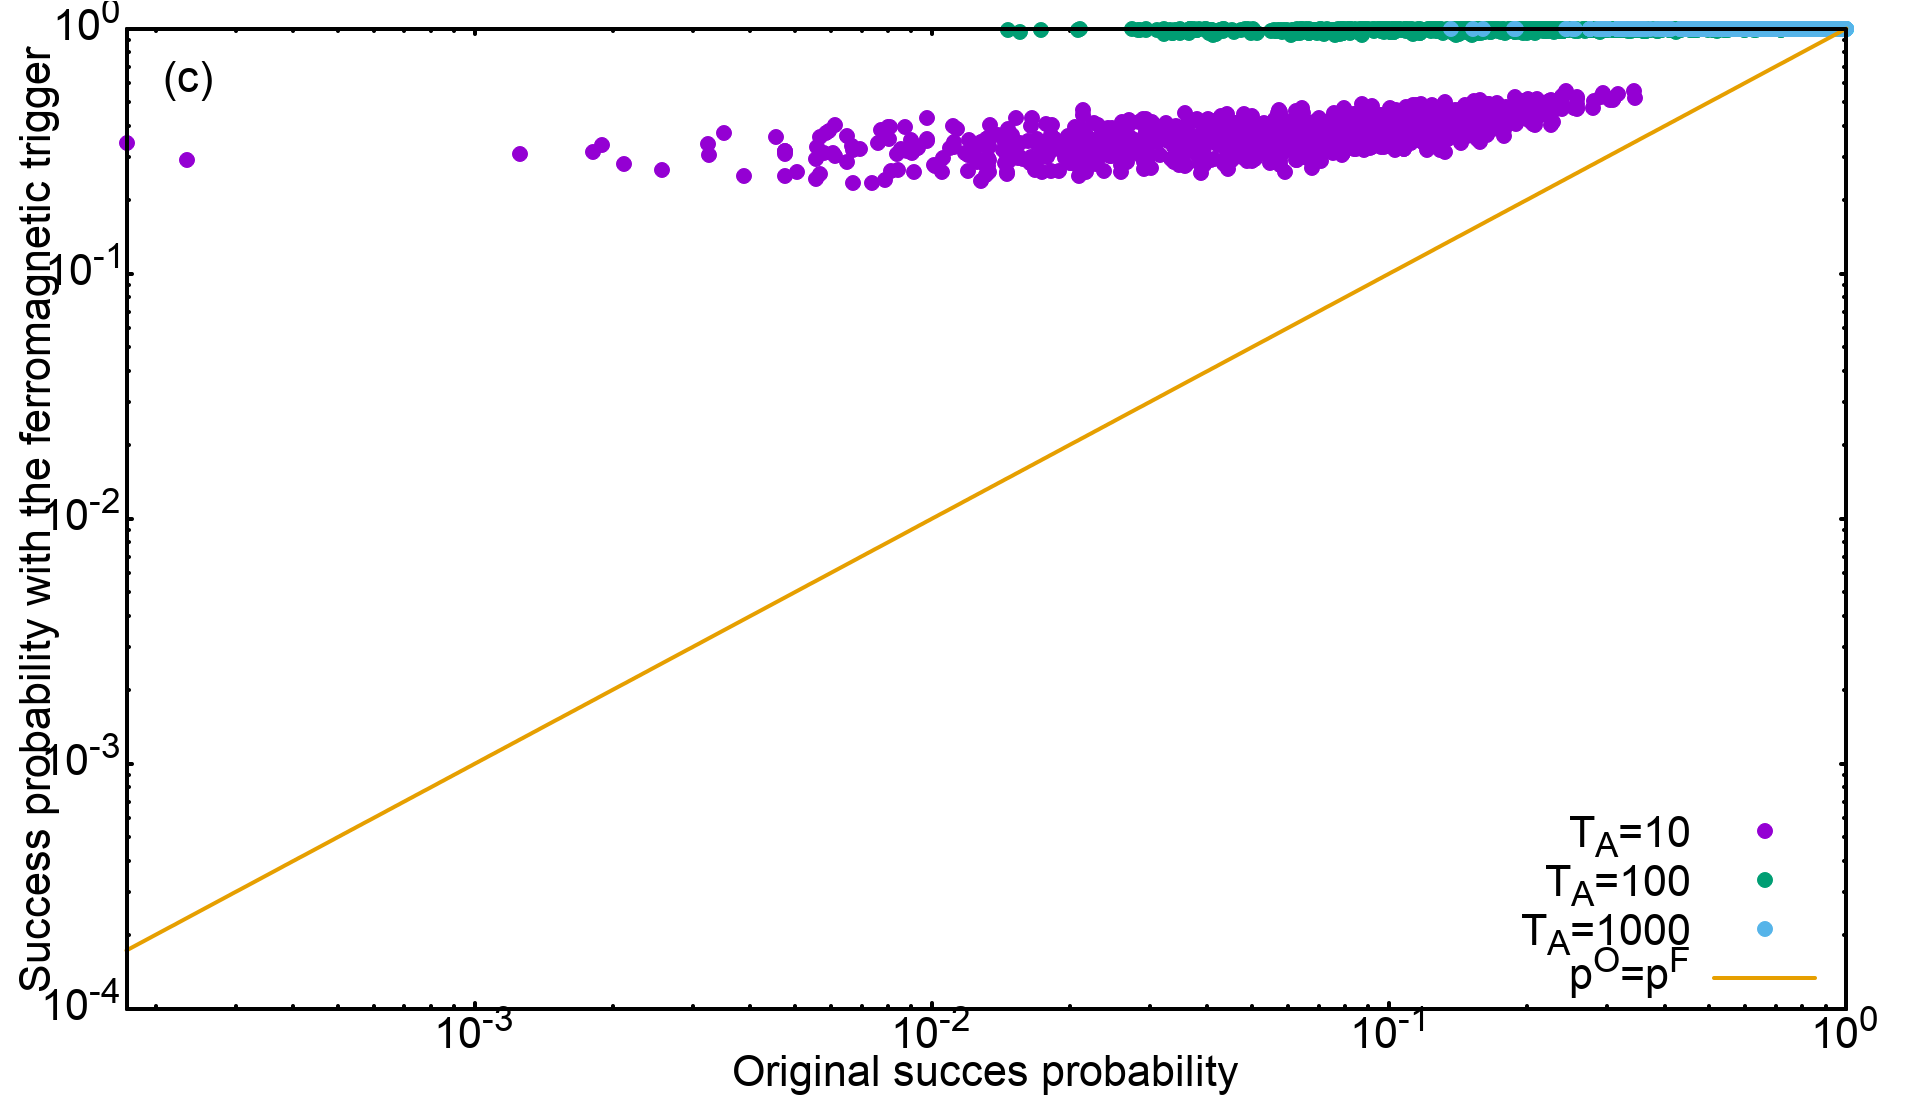
\includegraphics[scale=0.24]{Scatt_s12_F_g2.png}
\caption{Scatter plot for the success probability after adding ferromagnetic trigger with g-=2 against the success probability of the original Hamiltonian, for annealing time $T_A \in \{10,100,1000\}$. The solid line represents the limit where the success probability remains unchanged.}
\label{fig:f13}
\end{figure}

For all the three cases, and all the problems in the set, the success probability after adding the trigger was found to be greater than the success probability of the original Hamiltonian. Since in the adiabatic regime, the overlap of the final state with the ground state increases with increasing the annealing times, the success probability of the original Hamiltonians with long annealing times ($T_A$=1000) is already large ($\approx$ 1). Adding the ferromagnetic trigger can therefore not improve the success probability too much. This explains the confinement of the points representing the success probability for $T_A$=1000 close to the solid line ($p^O=p^F$) on the upper right corner for all the three values of the strength parameter. Owing to the same reason, the points corresponding to the success probability for $T_A$=10 have a much larger spread. For the easy cases (larger $p^O$), the success probability upon adding the trigger ($p^F$) has a similar value. Such points lie close to the line. On the other hand, for more difficult cases (smaller $p^O$) the improvement can be larger, and such points lie away from the line.\\

Furthermore, since for a given problem, increasing the strength of the ferromagnetic trigger makes the minimum gaps larger, the success probability for that case also becomes larger. This explains the distribution of the points getting successively more flat with increasing strength of the trigger, for all annealing times (see Figs. \ref{fig:f11}, \ref{fig:f12} and \ref{fig:f13}).\\

Finally, we look at the dynamics of the evolution. According to Eq. (\ref{eq:lz3}), for an adiabatic evolution of the state of the system, the success probability, p, i.e. the measure of the overlap of the final state with the ground state of the Hamiltonian, is related to the minimum energy gap, $\Delta_{min}$ as follows:
\begin{equation}
p=1-exp(-C{\Delta_{min}}^2),
\end{equation}
for some constant C. Since different problems in the problem set correspond to different minimum energy gaps, a plot of the success probability with these gaps should follow Eq. (\ref{eq:lz3}) if the evolution of the state for a problem is adiabatic. Moreover, adding the trigger changes the energy spectra, and thereby the minimum energy gaps of these problems. Fig. (\ref{fig:f14}) shows the success probability versus the minimum energy gap plot for all the problems upon adding the ferromagnetic trigger with three different strengths (0.5,1 and 2), and for three annealing times (10,100 and 1000).

\begin{figure}[H]
\centering
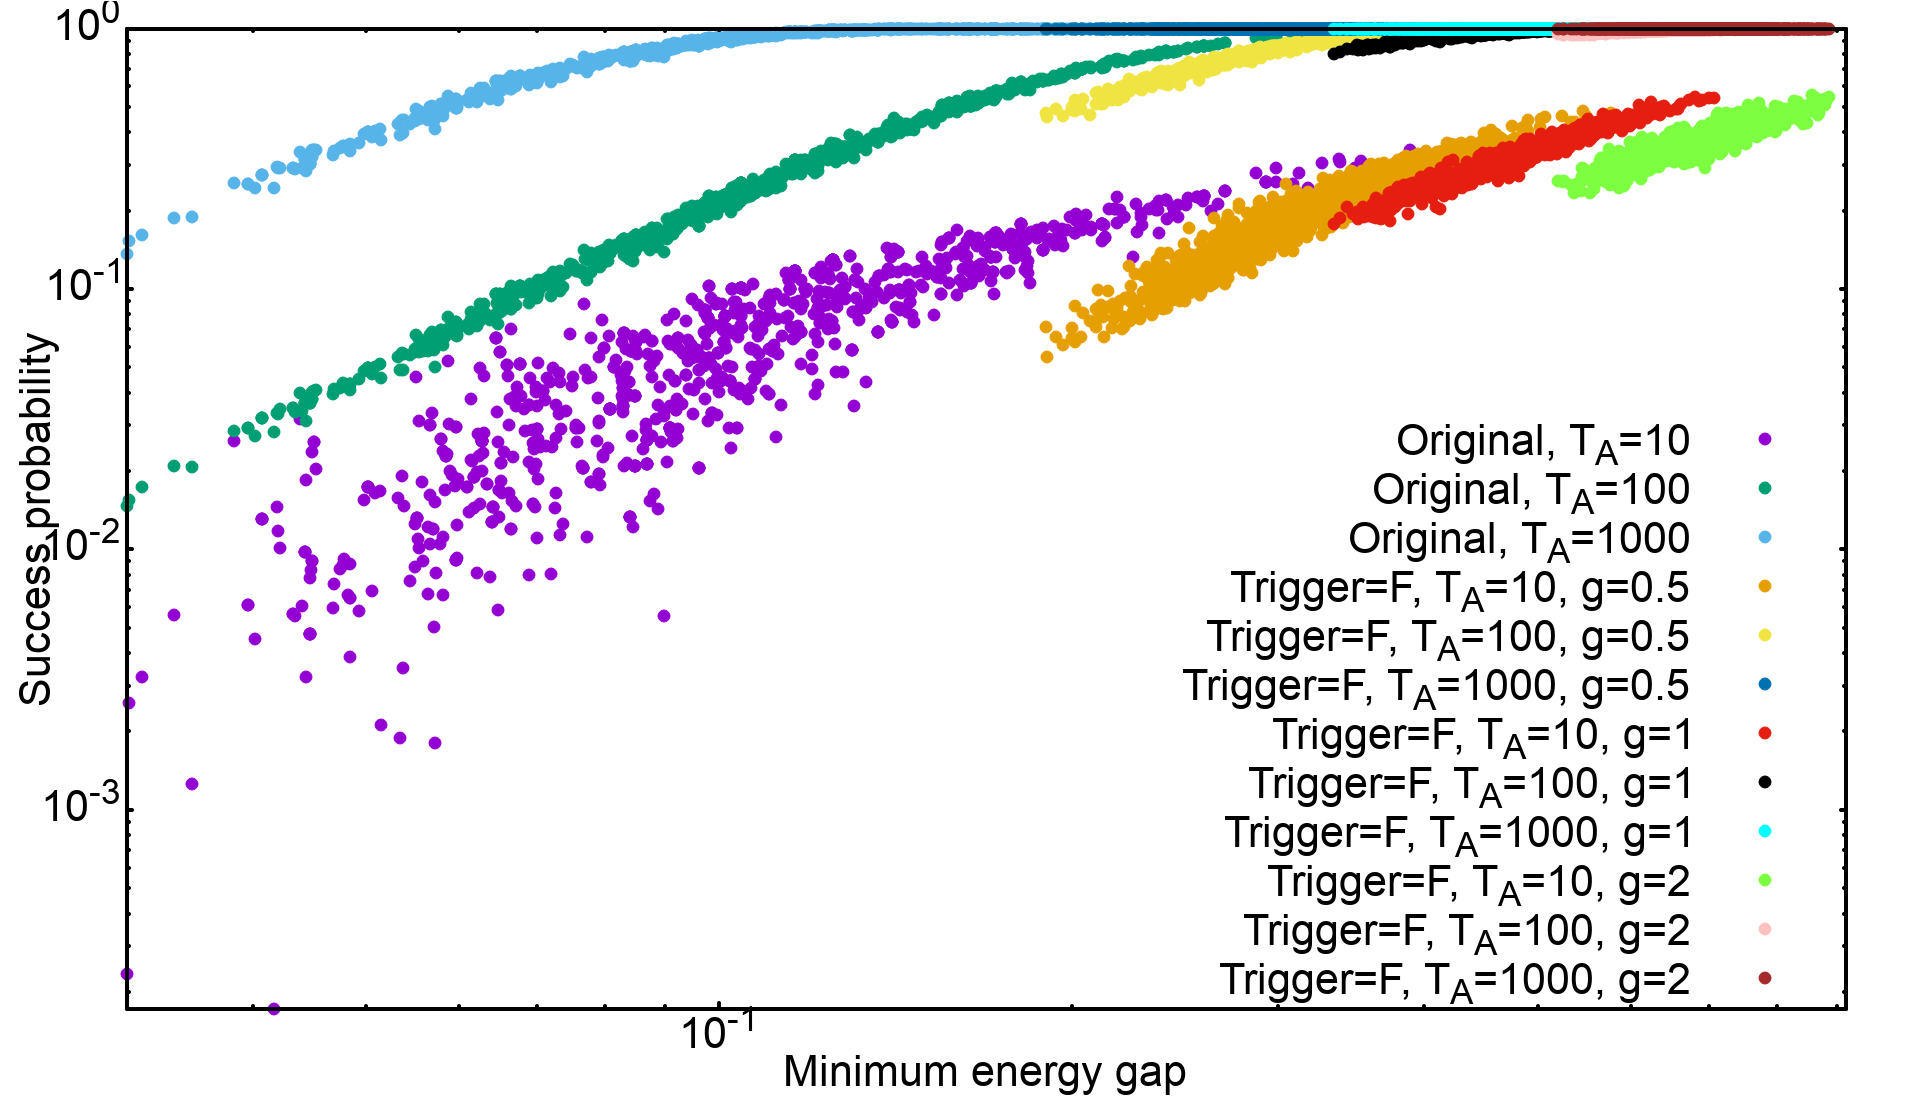
\includegraphics[scale=0.24]{SuccVsGap_OF_g.png}
\caption{Plot of the success probability versus minimum energy gaps for all the problems belonging to the set. The plot shows the effect of adding ferromagnetic trigger to the original Hamiltonian with strengths 0.5, 1 and 2, while the annealing time is chosen to 10, 100 and 1000.}
\label{fig:f14}
\end{figure} 

From the Fig.(\ref{fig:f14}) it can be noted that all the curves roughly follow the Landau-Zener dependence (see Eq. (\ref{eq:lz3})) of the success probability on the minimum energy gaps. However, for the original Hamiltonian, and $T_A$=10, the scattering is larger compared to the other curves. The scattering of the curves decreases on increasing the annealing times, suggesting that longer annealing times ascertain the evolution of the state to be adiabatic. Since adding the ferromagnetic trigger enlarges the minimum energy gaps, the curves are shifted to the right upon adding the trigger and increasing their strength. 
\end{document}